Climate change produced by greater atmospheric CO$_2$ concentrations
\cite{kane_atmospheric_1996} from human activity has led to increased exposure
to hazards worldwide and domestically: increased storm severity, rising sea
levels, more extreme temperatures, hotter summers, and rising sea levels to name
a few \cite{reidmiller_fourth_2018}. Without immediate action to reduce carbon
emissions, these impacts will worsen
\cite{intergovernmental_panel_on_climate_change_climate_2014}. Specifically, it
is primarily our societal dependence on fossil fuels to support our expansive
economies and energy systems that contributes the most to rising carbon dioxide
levels (along with other \acp{ghg}) \cite{epa_inventory_2023}. Therefore, to
achieve the almost universally shared goal of halting and reversing the effects
of climate change \cite{united_nations_paris_2015}, our globalized society must
transition away from fossil fuels to clean energy technologies such as nuclear
and renewable energy and switch our transportation systems to electric or
hydrogen powered vehicles
\cite{intergovernmental_panel_on_climate_change_climate_2021}. 

Naturally, the importance of modeling energy systems to gain insight and form
strategies to achieve this transition has grown. Especially since the spatial
and temporal complexities are also expected to grow with greater penetration of
\ac{vre}, such as solar and wind energy --- two energy sources that are
spatially diffuse and temporally challenging to predict. A class of tools called
\acp{esom} are the most common method for understanding our energy systems.
However, while climate change may be the most immediate existential threat to
society \cite{hickman_climate_2021}, it is a focusing issue that brings
challenges of equity and disproportional impacts to the fore. These latter
challenges have been always been concomitant with our energy system, but energy
system modeling has largely ignored the ways energy systems mediate
socio-political power alongside transporting electrons and fuel. For example,
fossil fueled power plants have always been associated with air pollution and
worsened health for nearby communities --- commonly poorer and black
communities, which are already marginalized, evincing a violation of fairness
and justice principles \cite{mohai_which_2015}. Studying these consequences of
our energy choices historically belonged to domain of the environmental justice
literature \cite{schlosberg_reconceiving_2004,mohai_environmental_2009} but has
developed further into the discipline of energy justice
\cite{sovacool_energy_2015}. 

The energy transition will require a great expansion of our energy
infrastructure to build replace fossil-fueled energy with clean energy and
additional transmission networks to carry electrons. Although the technology to
accomplish this transition is mature, there is still local public opposition to
many energy projects \cite{wolsink_wind_2007}. Particularly in empowered and
affluent communities \cite{stokes_prevalence_2023}. \acp{esom} cannot capture
these ``human dimensions'' of energy systems despite some awareness of their
importance \cite{pfenninger_energy_2014}. This is because they only optimize a
single objective --- cost (or some other aggregated economic metric). People
have and express preferences over many dimensions simultaneously. Further, even
in the absence of climate change, incorporating social context into the practice
of energy modeling remains beneficial since doing so will create substantively
better decisions \cite{wilsdon_see-through_2004}. The solution for enclosing
this feature of energy system design proposed in this thesis is two-fold. The
first is to develop an \ac{esom} capable of multi-objective optimization. The
benefits of multi-objective optimization have been understood for some time, yet
only recent advances in computing power have made them a practical method for
energy modeling. Hobbs (1995) wrote:

\begin{quote}
    Multi-objective methods are more appropriately used to help people to
    understand the problem better, explore their feelings, form a coherent,
    defensible set of values, and understand the implications of those values
    for the decision. [...] In reality, people's values are often uncertain and
    incoherent. During the course of a planning exercise, people's attitudes
    will evolve in response to new information, interactions with other people,
    and viewing the problem from different perspectives
    \cite{hobbs_optimization_1995}.    
\end{quote}

This leads to the second major proposal for this thesis, which is to validate
the multi-objective \ac{esom} developed within by conducting a case study in the
Champaign-Urbana region involving interviews with local energy planners and
incorporating their feedback to develop a planning process that encourages
greater participation by the community members. Altogether, this work will allow
``non-technical'' perspectives to be incorporated into a rigorous modeling
framework leading to greater perceptions of legitimacy through an iterative
articulation of values and priorities involving the public as key deliberators.
The result is a step towards a holistic integration of energy justice and energy
system engineering.

Chapter \ref{chapter:lit-review} discusses the existing literature and work from
several spanning disciplines, including risk assessment, energy justice, and
energy system optimization. Chapter \ref{chapter:methods} details the technical
methods I applied to create a flexible multi-objective optimization framework
called \ac{osier}. Chapter \ref{chapter:benchmark-results} validates \ac{osier}
as an \ac{esom} by comparing its results against an established representative
\ac{esom}, and demonstrates current progress. Finally, Chapter
\ref{chapter:proposal} outlines a proposal for the remaining work of this
thesis.

\section{Motivation}

\textcolor{red}{CO2 emissions}

\textcolor{red}{Emissions by energy source}

\section{Research Objectives}

\section{Reproducing this work}
Talk about \texttt{snakemake}, show the DAG... 

% \newpage
% \begin{landscape}
    \begin{figure}[h!]
        \centering
        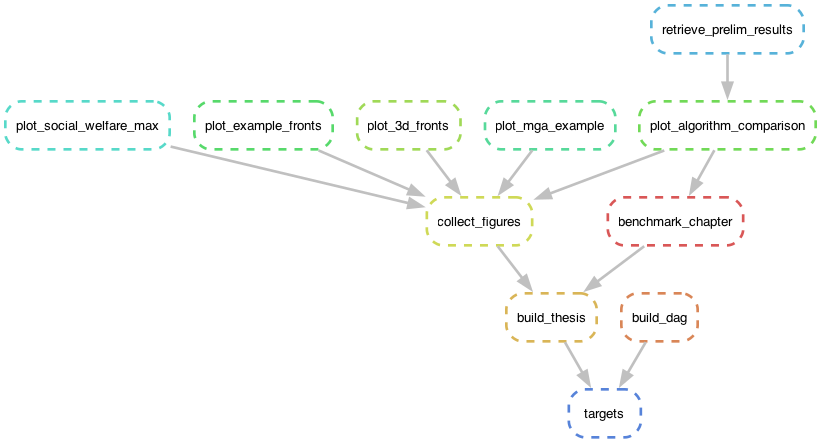
\includegraphics[width=\columnwidth]{../analysis/dag.png}
        \caption{The \ac{dag} illustrating the steps to produce this thesis.}
        \label{fig:dag}
    \end{figure}
% \end{landscape}